\chapter{Introducción}
El objetivo de este proyecto es construir un software con el que poder visualizar e interactuar con los datos DICOM obtenidos al someter a una escultura a una Tomografía Axial Computerizada (TAC). 

Para ello se hará uso de VTK, que proporciona una serie de librerías en C++ para facilitar operaciones sobre datos DICOM, y de Qt, para la Interfaz Gráfica de Usuario (GUI).

Antes de empezar con el proyecto en sí, se definirán conceptos como DICOM o TAC que se usarán a lo largo de éste y conviene saber lo que son, así como las distintas herramientas que se utilizarán.

\section{Obtención de datos DICOM mediante un TAC}
DICOM (\textit{Digital Imaging and Comunication in Medicine}) es el estándar internacional para manejar, visualizar, almacenar, imprimir y transmitir imágenes de pruebas médicas (ISO12052) \cite{about_dicom}. 

Al contrario de lo que se puede pensar en un principio, DICOM es más que un formato de imagen, es un protocolo que abarca la transferencia, el almacenamiento y la visualización \cite{dicom_intro_and_guide}.

Pese a que su uso está mayoritariamente extendido en el campo en el que nació (la medicina), se puede usar en otros, como el de la restauración de bienes culturales, como es el caso de este proyecto.

En un archivo DICOM hay almacenado, además de metadatos, una imagen \cite{dicom_classes_vtk} (Figura \ref{fig:prostate_dicom}).

\begin{figure}[H]
	\centering
	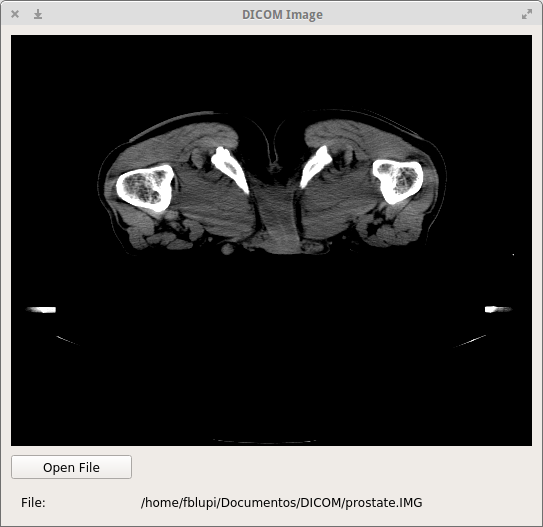
\includegraphics[width=10cm]{imagenes/prostate_dicom}
	\caption{Imagen DICOM de una próstata visualizada con un programa diseñado para visualizar archivos DICOM}
	\label{fig:prostate_dicom}
\end{figure}

\begin{figure}[H]
	\centering
	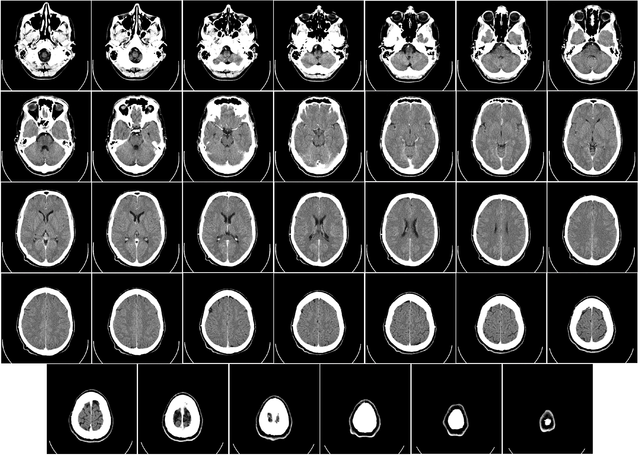
\includegraphics[width=10cm]{imagenes/brain_dicom_serie}
	\caption{Serie de imágenes DICOM extraídas de un TAC realizada a un cerebro}
	\label{fig:brain_dicom_serie}
\end{figure}

Cuando se realiza un escáner TAC (Tomografía Axial Computerizada) se obtiene una serie de imágenes (Figura \ref{fig:brain_dicom_serie}) de rebanadas del objeto al que se le realiza el escáner. Éstas imágenes se encapsulan en archivos DICOM, y con todas ellas se puede llegar a construir un modelo volumétrico.

El cómo se obtienen las imágenes con un TAC no es objeto de estudio de este proyecto, por lo que no se entrará en mucho detalle. En muy resumidas cuentas, el aparato emite un haz de rayos X desde distintos ángulos al objeto y unos sensores recogen la radiación que absorbe en cada una de estas emisiones. Obteniendo el resultado final del promedio de todas las mediciones que realizan los sensores \cite{tac}. 